

Альтернативным решением проблемы напыления атомов Tm на зеркало, находящееся перед пучком,  было проектирование источника атомов, не использующего для охлаждения атомарного пучка встречный лазерный луч. Одним из вариантов реализации такого источника является конфигурация 2D-МОЛ. В данной главе делаются оценки на возможный поток загрузки МОЛ $\sub{\Phi}{load}$, который можно получить с помощью 2D-МОЛ. Конструкция подразумевает, что из печи атомы попадают сразу в 2D-МОЛ, где плоскость 2D-МОЛ содержит и источник атомов (рис. \ref{fig:2dmots}). Затем в поперечном к 2D-МОЛ направлении атомы выталкиваются c помощью толкающего луча и так долетают до основной МОЛ. 


\begin{figure}[ht]
    \centering
    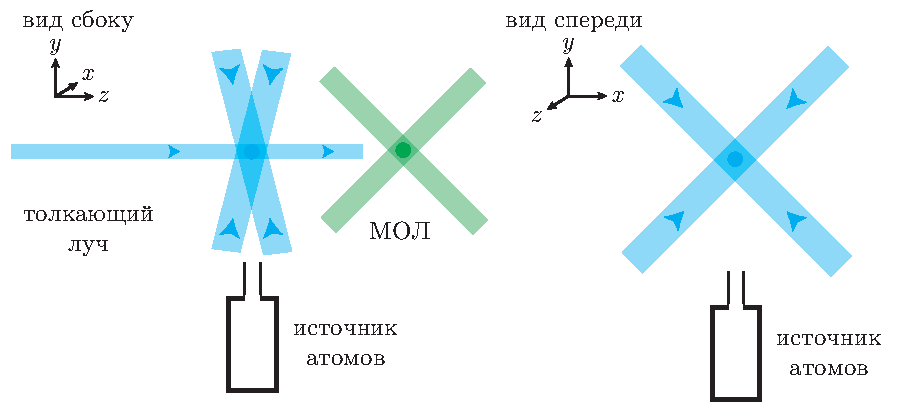
\includegraphics{figs/2dmot_v2.pdf}
    \caption{Принципиальная схема лучей 2D-МОЛ}
    \label{fig:2dmots}
\end{figure}
